%\documentclass{nature}
\documentclass{article}
\usepackage[english,american]{babel}
\usepackage[backend=biber,style=nature]{biblatex}
\usepackage[disable]{todonotes}
\usepackage{grffile}
\usepackage{booktabs}
\usepackage{hyperref}
\usepackage{graphicx}
\usepackage{fullpage}
%\usepackage{algorithm}
%\usepackage{algorithmic}
\usepackage{amsmath}
%\usepackage{subcaption}
%\usepackage{multicol}
\usepackage{csquotes}
\usepackage{pdfpages}
\usepackage{placeins}

\renewcommand{\vec}[1]{\mathbf{#1}}

%\renewcommand{\includegraphics}[2][]{\fbox{}}

\addbibresource{connectomics motif.bib}
\addbibresource{connectomics motif-relational models.bib}

\DeclareGraphicsRule{.ai}{pdf}{.ai}{}


\title{Automatic discovery of circuit structure from neural connectomics}
\author{Eric Jonas$^1$, Konrad Kording$^{2, 3,4}$}

\begin{document}
\maketitle

\begin{small}
\begin{enumerate}
  \item Department of Brain and Cognitive Sciences, Massachusetts Institute of Technology, Cambridge, Massachusetts
  \item Department of Physical Medicine and Rehabilitation, Northwestern University and Rehabilitation Institute of Chicago, Chicago, Illinois
  \item Department of Physiology, Northwestern University, Chicago, Illinois
  \item Department of Applied Mathematics, Northwestern University, Chicago, Illinois
\end{enumerate}
\end{small}

\begin{abstract}
  New techniques produce massive data about neural connectivity,
  necessitating new analysis methods to discover the biological and
  computational basis of this connectivity. It has long been assumed
  that discovering the local patterns of microcircuitry is the key to
  understanding neural function. Here we developed a nonparametric
  Bayesian technique that identifies neuron types and microcircuitry
  patterns in connectomics data. We show that the approach recovers
  known neuron types in the retina, reveals interesting structure in
  the nervous system of c. elegans, and automatically discovers the
  structure of microprocessors. Our approach extracts structural
  meaning from connectomics, enabling new approaches of deriving
  anatomical insights from these emerging datasets.


\end{abstract}

\section*{Introduction}
Emerging techniques \autocite{Morgan2013,Zador2012} promise to
quantify the location of each neuron within a volume of interest,
along with its connections to all other neurons. Far exceeding the
capacity of neuroanatomists to trace small circuits, this leads to
enormous datasets that quantify aspects of the nervous system. The impact of
this kind of high-throughput transition has been seen before -- 
rise of sequencing techniques necessitated the
development of novel computational methods to understand genomic
structure, ushering in an era of bioinformatics as an independent
discipline \autocite{Koboldt2013}.

The brain consists of multiple kinds of neurons, each of which is
hypothesized to have a specific role in the overall
computation. Neuron types differ in many ways, e.g. chemical or
morphological, but they also differ in the way they connect to one
another. In fact, the idea of well defined local connectivity patterns
(microcircuits) has been prominent in many areas, ranging from sensory
(e.g. retina, \autocite{Masland2001} via processing (e.g. neocortex
\autocite{Mountcastle1997}) to movement (e.g. spinal cord)
\autocite{Grillner2005}. Indeed, such repeated patterns also exists in
human-made computing circuits. It remains an important challenge to
develop algorithms to use anatomical data, e.g. connectomics, to back
out underlying microcircuitry.

The discovery of structure is a crucial aspect of network
science. Early approaches focused on global graph properties, such as
the types of scaling present in the network \autocite
{WattsStrogatz1998} .  While this approach leads to an understanding
of global network, more recent work aims at identifying very small-scale
repeat patterns, or “motifs” in networks\autocite{Milo2002}

The discovery of structure in probabilistic graphs is a crucial aspect
in machine learning. Commonly used algorithms include
community-based-detection methods \autocite{Girvan2002}, and
stochastic block models \autocite{Nowicki2001}.  While these
approaches can incorporate the probabilistic nature of neural
connections \autocite{Hill2012} they do not generally consider the
known fact that the probability of connections between neurons depends
on distance. Combining such probabilistic models with a spatial
component to model distance promises to improve the detection of
microcircuitry from neural data.

When it comes to neuroscience and other computing systems, we expect
patterns of connectivity much more complex than traditional motifs,
exhibiting a strong spatial dependence arising from the complex
genetic, chemical, and activity-based neural development process. 


Here we describe a Bayesian non-parametric model that can discover
circuit structure automatically from connectomics data: both the cell
types and their spatial patterns of interconnection. We apply it to
three computing systems: the mouse retina connectome
\autocite{Helmstaedter2013}, the c. elegans connectome
\autocite{White1986}, and a ``connectome'' of a classical
microprocessor \autocite{James2010}. Note we do not explicitly
consider cellular morphology, absolute position (cell layer), or any
chemical or genetic information. Yet in all cases, we discover
cell-type to cell-type connectivity that depends on spatial distance
and these connectivity functions depend on the two involved cell
types. Comparing the cell types discovered by the algorithms with
those obtained by anatomists based on orthogonal information reveals a
high degree of agreement. We present a scalable approach to infer
microcircuitry from connectivity data.

\begin{figure}
  \centering 
  \centerline{\includegraphics[width=183mm]{overview.ai}}
  \caption{An overview of our method. a. Input data is
a connectivity matrix indicating whether cell $i$ (row)
synapses on cell $j$ (column). The location of each cell in space is known. 
b. Our algorithm discovers hidden cell types in this connectivity data
by assuming all cells of a type share a distance-dependent connectivity 
profile, c.), with cells of other types. This results in a clustering 
of the cells by those hidden types. b.) shows the cell connectivity
matrix with cells of the same type grouped together. d.) shows
the learned probability of connection between our different types
at various distances, illustrating short-range and long-range
connectivity patterns.}
\label{fig:overview}
\end{figure}

\section{Results}
We use a Bayesian structure discovery approach that is based on prior
knowledge about the way positions and cell types affect the
probability of connections between cells, a so-called generative
model. Basing our model on previous infinite stochastic block models
(iSBM)\autocite{Kemp2006a,Xu2006}, we assume that each neuron is a
member of a single ``type'', and that the probability of two neurons
being connected is a function of their types. Crucially, we
incorporate the prior knowledge that spatial proximity matters, adding
distance-dependence to the iSBM.  For example, retinal ganglion cells
may synapse on nearby, but not far away, amacrine cells.  Note that
this simplistic prior information is all that we tell our model; no
additional physiological information is included.  We term our model
the ``infinite spatial-relational model'' (iSRM), in keeping with the
existing nonparametric literature, as it discovers a potentially
unbounded number of unobserved, or ``latent'', cell types.

We combine annealing with Markov Chain Monte Carlo to
perform simultaneously joint posterior inference over the structure,
parameters, and hyperparameters of the model (see Methods). This
procedure automatically learns the number of cell types, which cells 
belong to which types, along with the 
the distance and type dependent connectivity probabilities (see
fig~\ref{fig:overview}). These results can then be compared with the
results of previous anatomical studies that have used other aspects of
neurons, such as chemical properties and cell-morphology to divide
neurons into types.

Before we can use a probabilistic model to analyze real data we first
need to assess if the model works properly. We thus started out by
simulating data for which we know the correct structure and comparing
the estimated structure based on the algorithm (see methods) with the
one we used for simulation. We find that the model does a good job of
recovering the correct number of cell types,
(fig~\ref{fig:synthetic}a), the the cell identities
(fig~\ref{fig:synthetic}b), and the spatial extent of each type
(fig~\ref{fig:synthetic}c).  Indeed, it does far better than the
existing infinite stochastic block model that assumes that there is no
distance dependence to the connectivity. The model converges
relatively quickly to an estimate of the most probable values for the
cell types, which is enabled by using a combination of simulated
annealing and parallelized Markov chain Monte Carlo (see methods for
details). It appears that the model behaves the way it should and
allows application to relatively large datasets.

\begin{figure}
  \centering 
  \centerline{\includegraphics{synthetic.ai}}
  \caption{Correct recovery of true numbers of hidden classes
in synthetic data. a.) The iSBM over-segments the number
of classes as it fails to take distance into account, whereas
our model finds close to the true number of classes. b.) ARI, a measure
of ``correct clustering'', for
different true class counts, between our model and a traditional
iSBM. c.) For synthetic data, 
the iSBM overclusters, finding a large number of spatially-localized types. 
In contrast, the infinite spatial-relational model recovers the true spatial
extent of the underlying types.}
\label{fig:synthetic}
\end{figure}

\subsubsection{Mouse Retina}

\begin{figure}
  \centering 
  \centerline{\includegraphics{mouseretina.ai}}
  \caption{Discovering cell classes in the mouse retina connectome. 
a.) Input connectivity data for 950 cells for which soma positions were known. b. clustered connectivity matrix. c.) connectivity diagram showing our clusters, as
well as the cell depth and known cell type of each cell. Our model agrees
with the cell types traditionally identified by anatomists, and identifies 
laminar-specific connectivity patterns. d.) Connectivity between our
clusters as a function of distance -- the cluster consisting primarily of
retinal ganglion cells (lower left-center) exhibits the expected near and
far connectivity. e. The spatial distribution of our cell types -- each cell type tesselates space.}
\label{fig:mouseretina}
\end{figure}

The retina of the mouse \autocite{Masland2001} is an example where we
should expect to have connectivity patterns that are well approximated
by our generative model. It is known that there are multiple classes
of cells that can be grouped into ganglion cells that transmit
information to the rest of the brain, bipolar cells that connect
between different cells, and amacrine cells that feed into the
ganglion cells \autocite{cite some review}. Recent research
\autocite{Helmstaedter2013} has produced a large dataset containing
both the types of cells from orthogonal approaches, and also the
connectivity matrix between all reconstructed cells. We want to know
to which level we can classify neurons into types based on this
connectivity only.

The algorithm took 8 hours to converge to a locally optimal solution,
dividing neurons into a set of cell types (fig~\ref{fig:mouseretina}c, each
wedge is a type). For each pair of neurons there is a specific
distance dependent connection probability (fig~\ref{fig:mouseretina}b,c,d),
which is well approximated by the model fit. Moreover, each type of
cell is rather isotropically distributed across space
(fig~\ref{fig:mouseretina}e) as should be expected for true cell types. The
algorithm is thus able to extract meaningful structure from the data.

Comparing the results of the algorithm to other information sources
allows evaluating the quality of the type determination. Our types
closely reflect the (anatomist-determined) segmentation of cells into
retinal ganglion, narrow amacrine, medium/wide amacrine, and bipolar
cells (fig~\ref{fig:mouseretina}c, outermost ring). We find that the
types we find tend to reflect the known laminar distribution in the
retina (fig~\ref{fig:mouseretina}c, middle ring), which is exciting as
the algorithm did not actually use this type of information.


The algorithm yields a separation of neurons into a smaller number of
types than the fully granular listing of 71 types found by the
original authors of the paper, although is still highly correlated
with those finer type distinctions (see
supp~\ref{supp:mouseretina}. It is our expectation that, with larger
datasets, even closer agreement would be found.

\todo{Do we assign any of the unknown cells correctly?  are types 72-79
“different” or simply unknown?}

We compared the results of our model to the traditional iSBM to see if
the addition of spatial information was necessary. We find that, as
expected from our synthetic experiments, the iSBM massively
over-segmented the data, finding spatially-localized “communities” of
cells which bore little relation to known types.  The average spatial
extent of the types found by the iSBM was $14.6\pm8.1 \mu m$. Using
the anatomists' ground truth, the mean spatial extent of types was
$34.3\pm7.6 \mu m$, quite close to the $34.5\pm 1.0 \mu m$ discovered
by our algorithm. Modeling the distance-dependence prevents
over-segmentation and thus allows more meaningful estimates.

% from experiments/mouseretina/spatial_var.txt

% Relational Model: mean = 14.586508 std=8.136334
% Spatial-Relational Model: mean = 34.540355 std=1.069483
% Truth (fine): mean = 34.348443 std=7.567564
% Truth (coarse): mean = 35.276636 std=2.372951

\subsection{C. elegans}

The roundworm Caenorhabditis elegans is a model system in
developmental neuroscience\autocite{White1986}, with the location and
connectivity of each of 302 neurons deterministically known. This
incredible cross-organism consistency led to early mapping of the
c. elegans chemical and electrical (gap junction) connectome. Unlike
the retina, only the motor neurons in c. elegans exhibit regular
distribution in space, being distributed along the body axis. Most
interneurons are concentrated in various ganglia that project
throughout the entire animal, and the sensory neurons are primarily
located in a small number of anterior ganglia. 

\begin{figure}
  \centering 
  \centerline{\includegraphics[width=5in]{celegans.ai}}
  \caption{Discovering cell types in the \textit{c. elegans}
    connectome. a.) Initial cell connectivity matrix, red are
    (directional) chemical synapses, blue are electrical
    synapses. Point size is proportional to synapse count between
    those cells. b.) Clustered adjacency matrix showing identified
    clusters. c.) Inter-cluster connectivity, showing the position of
    each cell along the body axis as well as the ``true'' cell type --
    both coarse (motor, sensory, and interneuron) as well as fine
    (small text labels). }
  \label{fig:celegans}
\end{figure}

Using both the chemical and electrical connectivity (see methods), we
determined the underlying clusters explained by connectivity and
distance (fig~\ref{fig:celegans}a). A superficial inspection of the results shows
clustering into groups consisting roughly homogeneously of motor
neurons, sensory neurons, and interneurons. Closer examination reveals
agreement with the classifications originally outlined by Brenner in
1986.  

We identify cell types that reflect the known motor/non-motor neuron
classes, even though this system lacks the strong repeat
microcircuitry our model was designed for.  Motor-neuron types AS, DA,
VA, and VB are clustered together, 

as are


``The processes of VDn and DDn do not have extended, apparently undifferentiated distal regions, as do the other motoneuron classes; instead, they end abruptly in close proximity to the end of a neighbouring process of the same class, often with a gap junction between them''

motor-neuron types VD and DD, and head motor neuron types RMD and SMD. 

Various head motor neurons, including types
SMD, RMD, and RIM are clustered together. Interneurons with known
anatomically-distinct connectivity patterns, such as RIA (2 cells) or
AVA/AVB (4 cells) are clustered into pure types. 


Note our
clustering does not perfectly reflect known divisions -- several
combinations of head and sensory neurons are combined, and a
difficult-to-explain group of 2 VD, 2 VB, a VA, and a DD neuron are
grouped together. Our identified cell types thus reflect a
``coarsening'' of known types, based entirely on connectivity and
distance information, even when the organism exhibits substantially
less spatial regularity than the retina. 


\subsection{Microprocessor}
\begin{figure}
  \centering 
  \centerline{\includegraphics{mos6502.ai}}
  \caption{Discovering transistor types in the MOS 6502
    microprocessor. a.) The clusters and connectivity versus distance
    for connections between Gate and C1, Gate and C2, and C1 and C2
    terminals on a transistor. Red and teal types have a terminal
    pulled down to ground and mostly function as inverters. Purple
    class are clocked, stateful transistors, orange control the ALU
    and yellow control the special data bus. b.) The spatial
    distribution of the transistors in each cluster. }
\label{fig:mos6502}
\end{figure}

To show the applicability of our method to other connectome-style
datasets, we obtained the spatial location and interconnectivity of
the transistors in a classic microprocessor, the MOS Technology 6502
(used in the Apple II) \autocite{James2010}. Computer architects use
common patterns of transistors when designing circuits, with each
transistor having a ``type'' in the circuit. We identified a region of
the processor with complex but known structure containing the primary
8-bit registers X, Y, and S (fig~\ref{fig:mos6502}).

Our algorithm identifies areas of spatial homogeneity that mirror the
known structure in the underlying architectural circuit, segmenting
transistor types recognizable to computer architects. Using the
original schematics, we see that one identified type contains the
``clocked'' transistors, which retain digital state. Two other types
contain transistors with pins C1 or C2 connected to ground, mostly
serving as inverters.  An additional identified type controls the
behavior of the three registers of interest (X, Y, and S) with respect
to the SB data bus, either allowing them to latch or drive data from
the bus. The repeat patterns of spatial connectivity are visible in
figure~\ref{fig:mos6502}a, showing the man-made horizontal and
vertical layout of the same types of transistors.





\section{Discussion}
We have presented a machine learning technique that allows cell types
and microcircuitry to be discovered using only distance and
connectivity data. We have shown its applicability to a newly
published connectomics dataset from the mouse retina, the classical
connectivity of the worm c. elegans, and the connectivity of a
historical man-made microprocessor. We have found that distance and
connectivity alone are sufficient to discover cell types and
microcircuitry that were known to exist in the systems based on decades
of previous research which had utilized extensive additional
information.

For probabilistic models like ours, no known solution exists to
exactly find the most probable parsing of the neurons into cell-types
and connectivity patterns . We employ a collection of Markov-chain
Monte carlo techniques (see Methods) but while different
initializations converge to similar ultimate values, we can never
realistically obtain the global optimum. There are a broad range of
techniques that may offer better approximations to the global optimum
\autocite{Wanga2012} and future work could adapt them to
the problem we addressed here.

Our inference becomes slower as the amount of data increases. Our
algorithm required 30 hours for 1000 neurons and could take months for
substantially longer datasets. Scaling this class of probabilistic
model is an active area of research, and recent results in both
variational methods \autocite{Hoffman2013} and spectral learning
  \autocite{Anandkumar2012} promise substantial speed increases.

  Larger datasets will allow algorithms to distinguish more distinct
  types \todo{Add supplemental data} and we expect closer agreement
  with existing anotomical knowledge as more data become available.
  Moreover, in general, for such problems precision increases with the
  size of the dataset and the cells that we have are not sufficient to
  statistically distinguish all the cell types known in anatomy (such
  as the $\sim 70$ in the retina). Still, using only connectivity and
  distance it is possible to meaningfully divide neurons into types.

Our small collection of hand-selected distance-dependent likelihood
functions are clearly non-exhaustive, and assume monotonicity
of connectivity probability -- for a given class, closer cells
are never less-likely to connect. This is known to be insufficient
for various neural systems. Future models could incorporate
a wider variety of likelihood functions, or even learn the global
functional form from the data. 

There exist a range of previous approaches to the discovery of
neural microcircuitry \todo{Do we want a citation here?}. These
generally involve a great deal of manual labor and ad-hoc
determination of what constitutes a “type” of cell -- to this day
there are disagreements in the literature as to the “true” types in
the mammalian retina. Much as phylogenomics has changed our
understanding of animal ontologies, modern large scale data will allow
the efficient unbiased discovery of cell types and circuits. The sheer
amount of available data demands the introduction of algorithmic
approaches.

The development of automatic identification and quantification of cell
type may also provide a new computational phenotype for quantifying
the effect of disease, genetic interventions, and
developmentally-experienced neural activity. Our method can in
principle identify neuron-types across non-connected graphs,
e.g. across animals. For example, the types of neurons in one animal
can be associated with the types of neurons in another animal, in the
same way as this is already possible through molecular markers
\autocite{Brown2009}. This could be particularly important if cell
types appear that are due to properties of the stimuli and experience
as opposed to just the molecular properties of cells, such as color
and orientation selective types in primary visual cortex
\autocite{Sincich2005,Lennie2005}. This would allow comparative
quantitative anatomy across animals, and aid the search for the
ultimate causes of connectivity.

Ultimately, we will need to combine information across different
sources into a joint understanding of neural function. Distinct cell
types differ in morphology, connectivity, transcriptomics, relation to
behavior or stimuli and many other ways. Algorithms based on each type
information can then be combined to synthesize all the available
information from one experiment or even across experiments into a
joint model of brain function.

\subsection{Methods Summary}

We take as input a connectivity matrix $R$ defining the connections
between cell $e_i$ and $e_j$, as well as a distance function $d(e_i,
e_j)$ representing a (physical) distance between adjacent cells. See
the supplemental material for extension to multiple connectivity
matrices. We assume there exist an unknown number $K$ of latent
(unobserved) cell types, $k \in \{1, 2, 3, \dots, K\}$, and that each
cell $e_i$ belongs to a single cell type. We indicate a cell $e_i$ is
of type $k$ using the assignment vector $\vec(c)$, so $c_i = k$. The
observed connectivity between two cells $R(e_i, e_j)$ then depends
only on their latent type and their distance through a link function
$f(\cdot, d(e_i, e_j))$. We assume $f$ is parameterized based on the
latent type, $c_i=m$ and $c_j=n$, via a parameter$\eta_{mn}$, as well
as a set of global hyper parameters $\theta$, such that the link
function is $f(d(e_i, e_j) | \eta_{mn}, \theta)$. 

We then jointly infer the maximum a posteriori (MAP) estimate of the
class assignment vector $\vec(c) = \{c_i\}$, the parameter matrix $\eta_{mn}$, and
the global model hyperparameters $\theta$ :

\begin{equation}
  p(\vec{c}, \eta, \theta | R ) \propto \prod_{i, j} p(R(e_i, e_j) | f(d(e_i, e_j) | \eta_{c_ic_j}), \theta) \prod_{m, n} p(\eta_{mn} | \theta)  p(\theta) p(\vec{c} | \alpha) p(\alpha) p(\theta)
\end{equation}

Inference is performed in three steps via composible transition 
kernels -- one for structural, one for per-type parameters, and
one kernel for global parameters and hyperparameters. Details
of data preprocessing, inference parameters, and runtime can
be found in the Methods section. 

\printbibliography

\begin{itemize}

 \item \textbf{Acknowledgments} We thank Josh Vogelstein for discussions and reading of the manuscript, Finale Doshi-Velez for early discussions on the model, and Erica Peterson, and Jonathan Glidden for extensive manuscript review. Funding for compute time was provided by Amazon Web Services ``AWS in Education'' grants. 
\item \textbf{Author Contributions} KK and EJ developed model. EJ derived inference, implemented code, tested, and ran experiments. KK and EJ wrote manuscript text and solicited feedback. 
 \item \textbf{Competing Interests} The authors declare that they have no
competing financial interests.
 \item \textbf{Correspondence} Correspondence and requests for materials
should be addressed to E.J.~(email: jonas@mit.edu).
\end{itemize}

\newpage
\section{Methods }

\subsection{Probabilistic Model}

Our model is a extension of the iSBM
\autocite{Kemp2006a,Xu2006} to incorporate spatial relations between entities,
inspired by attempts to extend these models with arbitrary
discriminative functions\autocite{Murphy2012}.

We take as input a connectivity matrix $R$ defining the connections
between cell $e_i$ and $e_j$, as well as a distance function $d(e_i,
e_j)$ representing a (physical) distance between adjacent cells. See
the supplemental material for extension to multiple connectivity
matrices. We assume there exist an unknown number $K$ of latent
(unobserved) cell types, $k \in \{1, 2, 3, \dots, K\}$, and that each
cell $e_i$ belongs to a single cell type. We indicate a cell $e_i$ is
of type $k$ using the assignment vector $\vec(c)$, so $c_i = k$. The
observed connectivity between two cells $R(e_i, e_j)$ then depends
only on their latent type and their distance through a link function
$f(\cdot, d(e_i, e_j))$. We assume $f$ is parameterized based on the
latent type, $c_i=m$ and $c_j=n$, via a parameter$\eta_{mn}$, as well
as a set of global hyper parameters $\theta$, such that the link
function is $f(d(e_i, e_j) | \eta_{mn}, \theta)$. 

We then jointly infer the maximum a posteriori (MAP) estimate of the
class assignment vector $\vec(c) = \{c_i\}$, the parameter matrix $\eta_{mn}$, and
the global model hyperparameters $\theta$ :

\begin{equation}
  p(\vec{c}, \eta, \theta | R ) \propto \prod_{i, j} p(R(e_i, e_j) | f(d(e_i, e_j) | \eta_{c_ic_j}), \theta) \prod_{m, n} p(\eta_{mn} | \theta)  p(\theta) p(\vec{c} | \alpha) p(\alpha) p(\theta)
\end{equation}


% Methods section 3000 words
% methods summary does not appear in the online text
% methods section can have no figures or tables [grrr]



We describe the spatial ``Logistic-distance Bernoulli''  function here,
and others in the supplemental material. 

% fixme class component, NOT class
The ``logistic-distance Bernoulli'' spatial model assumes that, if cell
$e_i$ is of type $m$ and cell $e_j$ is of type $n$, then $\eta_{mn}
= (\mu_{mn}, \lambda_{mn})$, and the probability that two cells $e_i$
and $e_j$ are connected is given by
\begin{eqnarray}
p^* &=& \frac{1.0}{1 + \exp \frac{d(e_i, e_j) - \mu_{mn}}{\lambda_{mn}}}\\
p &= & p^* \cdot (p_{max} - p_{min}) + p_{min}
\end{eqnarray}
where $p_{max}$ and $p_{min}$ are global per-graph parameters. 

We place an exponential priors on the latent parameters:
\begin{eqnarray}
 \mu_{mn} \sim \exp(\mu | \mu^{hp}) \\
\lambda_{mn} \sim \exp(\lambda | \lambda^{hp})
\end{eqnarray}

using  $\lambda^{hp}$ and $\mu^{hp}$ as global per-graph hyperparameters. 

We use a Dirichlet-process prior on class assignments, which allows
the number of classs to be determined automatically. In brief, for $N$
total cells, the probability of a cell belonging to a class is
proportional to the number of datapoints already in that class, $N_k$,
such that $p(c_i = k) \propto \frac{m_k}{N + \alpha}$ and the
probability of the cell belonging to a new class $k'$ is $p(c_i = k')
\propto \frac{\alpha}{N + \alpha}$. $\alpha$ is the global
concentration parameter -- larger values of $\alpha$ make the model
more likely to propose new classes. We grid the parameter $\alpha$ and
allow the best value to be learned from the data.


\subsection{Inference} 
We perform posterior inference via Markov-chain Monte Carlo (MCMC),
annealing on the global likelihood during the traditional burn-in
phase. MCMC transition kernels for different parts of the state space
can be chained together to construct a kernel whose ergodic
distribution is the target ergodic distribution over the entire state space. 

Our first transition kernel (``structural'') performs gibbs sampling 
of the assignment vector $p(\vec{c} | \eta, \theta, \alpha)$. 
The lack of conjugacy in our likelihood model makes an explicit 
evaluation of the conditional assignment probabilities impossible, 
motivating us to use an auxiliary variable method \autocite{Neal2000}
in which a collection of ephemeral classs are explicitly represented
for the duration of the Gibbs scan. 

We then employ a transition kernel to update the per-component
parameter values $\eta_{mn}$. Conditioned on the assignment vector
$\vec{c}$ and the model hyperparameters $\theta, \alpha$ the 
individual $\eta_{mn}$ are independent. We slice sample \autocite{Neal2003}
each component's parameters, choosing the slice width as a function
of the global hyperparameter range. 

The global hyper-parameters, both $\alpha$ and $\theta$, are allowed
to take on a discrete set of possible values. As $\theta$ is often a
tuple of possible values, we explore the cartesian product of all
possible values. We then Gibbs sample (our final transition kernel),
which is always possible in a small, finite, discrete state space.

We chain these three kernels together, and then globally
anneal on the likelihood from a temperature of $T=64$ down to 
$T=1$ over 300 iterations unless otherwise indicated, and
then run the chain for another $100$ iterations. 

To pick the MAP, we run up to $100$ simultaneous chains in parallel,
initialized from different random initial points in the state space,
and then pick the chain with the highest log likelihood. Early
experiments attempted to use the full ensemble of chains as an
estimate of the posterior but were abandoned due to the difficulty of
summarizing the posterior over such a complex state space, which is an
ongoing area of research in the probabilistic modeling community
\todo{cite more? missing}.


\todo{Validation: do we want to write extensively about posterior
  enumeration tests, etc. ? }


\subsection {Mouse Retina}
\label{supp:mouseretina}
Dense serial electron microscopy of a $114\mu m \times 80 \mu m $ area
in the mouse retina by \autocite{Helmstaedter2013} yielded a listing
of places where neurons come into contact. There were over 1000 cells
originally, and selected the $950$ for which the location of the soma
could be reconstructed from the provided cell plots (soma locations
were not provided by the study's authors in machine-readable
form). Ultimately this left a matrix between the total synapse-like
contact area between all pairs of 950 cells. Area was thresholded at
$0.5\mu m$, determined by hand, to yield a 950 $\times$ 950 entry
matrix that served as input to our algorithm. We measured the distance
between cells using the reconstructed soma centers, and used the
Logistic-Distance spatial relation. Hyperprior griddings are shown in
supplemental section \ref{supp:hyperpriors}.

\subsection{C. elegans}

We obtained the connectome of c. elegans from data published
previously \autocite{Varshney2011}, and isolated the 279 nonpharyngeal
neurons, with a total of 6393 chemical synapses and 890 gap junctions
originally cleaned up in \autocite{Chen2006}. A cell's position was
its distance along the anterior-posterior axis normalized between zero
and one. We used both networks, the chemical network as a directed
graph and the electrical network as undirected graph. We use the
synapse counts with the logistic-distance poisson likelihood, scaling
the counts by 4.0 to compensate for the Poisson's overdispersion.

\subsection{Microprocessor}
We extracted the connection graph for the transistors in the MOS6502
\autocite{visual6502source}. Each transistor has three terminals (gate,
source, drain), but the methods of the original dataset were unable to
consistently resolve which of the C1 and C2 terminals were source and
drain, leading to ambiguity in our encoding. We identified a region
consisting of three registers X, Y, and S via visual
inspection and focused our efforts there. We created a total of six
connectivity matrices by examining possible terminal pairings. One
graph, for example, $R^{gc_1}(e_i, e_j)=1$ if transistor $e_j$ and
$e_j$ are connected via pins $g$ and $c_1$. 


% \begin{addendum}
%  \item Put acknowledgements here.
%  \item[Competing Interests] The authors declare that they have no
% competing financial interests.
%  \item[Correspondence] Correspondence and requests for materials
% should be addressed to A.B.C.~(email: myaddress@nowhere.edu).
% \end{addendum}
\newpage
\section{Supplemental}

\subsection{Other Likelihoods}
\label{supp:otherlikelihoods}

We reparameterized the Logistic-Distance Bernoulli likelihood to
better capture the microprocessor data structure. We are explicitly
setting the maximum probability $p$ of the logistic function on a
per-component basis, drawing from a global $p \sim \operatorname{Beta}(\alpha_{hp},
\beta_{hp})$. Then $\lambda$ is set for each component as a global
hyperparameter, $\lambda$.

The ``logstic-distance Poisson'' spatial model is used to explicitly mode the count of synapses, $c$, between two neurons. The probability of c synapses between two neurons is distributed $c \sim \textrm{Poisson}(c | r)$, where $r$ (the ``rate'') is generated by a scaled logistic function (the logistic function has range $[0, 1]$. For each component $\eta_{mn}$ we learn both the threshold $\mu_{mn}$ and the rate scaling factor $r_{mn}$ Thus if for cells $m$ and $n$ are likely to have on average $20$ synases if they are closer than $5 \mu m$, then $\mu_{mn} = 5$ and $r_{mn} = 20$  " 

Thus the probability of $R(e_i, e_j) = c$ synapses between two cells $e_i$ and $e_j$ is given by:
\begin{eqnarray}
r^* &=& \frac{1.0}{1 + \exp \frac{d(e_i, e_j) - \mu_{mn}}{\lambda}}\\
r & = & r^* \cdot (r_{mn} - r_{min}) + r_{min} \\
R(e_i, e_j) \sim \textrm{Poisson}(c | r)
\end{eqnarray}

where $\lambda$ and $r_{min}$ are per-graph parameters. Per-component parameters $\mu_{mn} \sim \exp(\mu | \mu^{hp})$ and $r_{mn} \sim \exp(r_{mn} | r_{scale}^{hp})$. 

\subsection{Source code}

All source code and materials for running experiments can be
obtained from the project website, at \\

\href{http://spatialrelation.github.io }{http://spatialrelation.github.io}


\subsection{Extension to multiple graphs}
\label{supp:multigraph}
The model can handle multiple graphs $R^q$ simultaneously with a shared clustering by extending the likelihood to include the product of the likelihoods of the individual graphs. 

\begin{equation}
  p(\vec{c}, \{\eta^q\}, \{\theta^q\} | \{R^q\} ) \propto \prod_q \Bigg(\prod_{i, j} p(R^q(e_i, e_j) | f(d(e_i, e_j) | \eta^q_{c_ic_j}, \theta^q) \prod_{m, n} p(\eta^q_{mn} | \theta^q)  p(\theta^q) \Bigg) p(\vec{c} | \alpha) p(\alpha) 
\end{equation}

\FloatBarrier

\subsection{Microprocessor Netlist annotation}
\label{supp:mos6502netlist}
This is a matrix consisting of the different clusters of electrical nets for 
the registers, with the colors consistent with figure~\ref{fig:mos6502}. 

\includepdf[pages=-]{mos6502.clusters.pdf}

\FloatBarrier
\subsection{Model Comparison for Mouse Retina}

We compare the classs found by our model, the traditional infinite
stochastic block model, and a finite stochastic block model with the number
of classes set to the best-found number from our iSRM model ($k=12$).

We see from fig~\ref{fig:supp:irmspatialcomparemouse} that the spatial
variance of our classes closely matches the ground truth, while the
other two models find spatially-localized
classs. Figure~\ref{fig:supp:mousecompareari} shows the ARI of our
clustering, the clustering found by the iSBM,
as well as the result of parametrically varying the traditional stochastic
block model for various values of $k$. 

The actual clusterings for iSRM, the iSBM, and $SBM_{k=12}$ are shown
in figures \ref{fig:supp:retinabbclusters},
\ref{fig:supp:retinaldclusters}, and
\ref{fig:supp:retinabbfixedclusters} respectively. Each block is a
cluster, with the true cell type indicated along the x-axis, and the
cell ID written to the left or right.


\begin{figure}[h!]
  \centering 
    \centerline{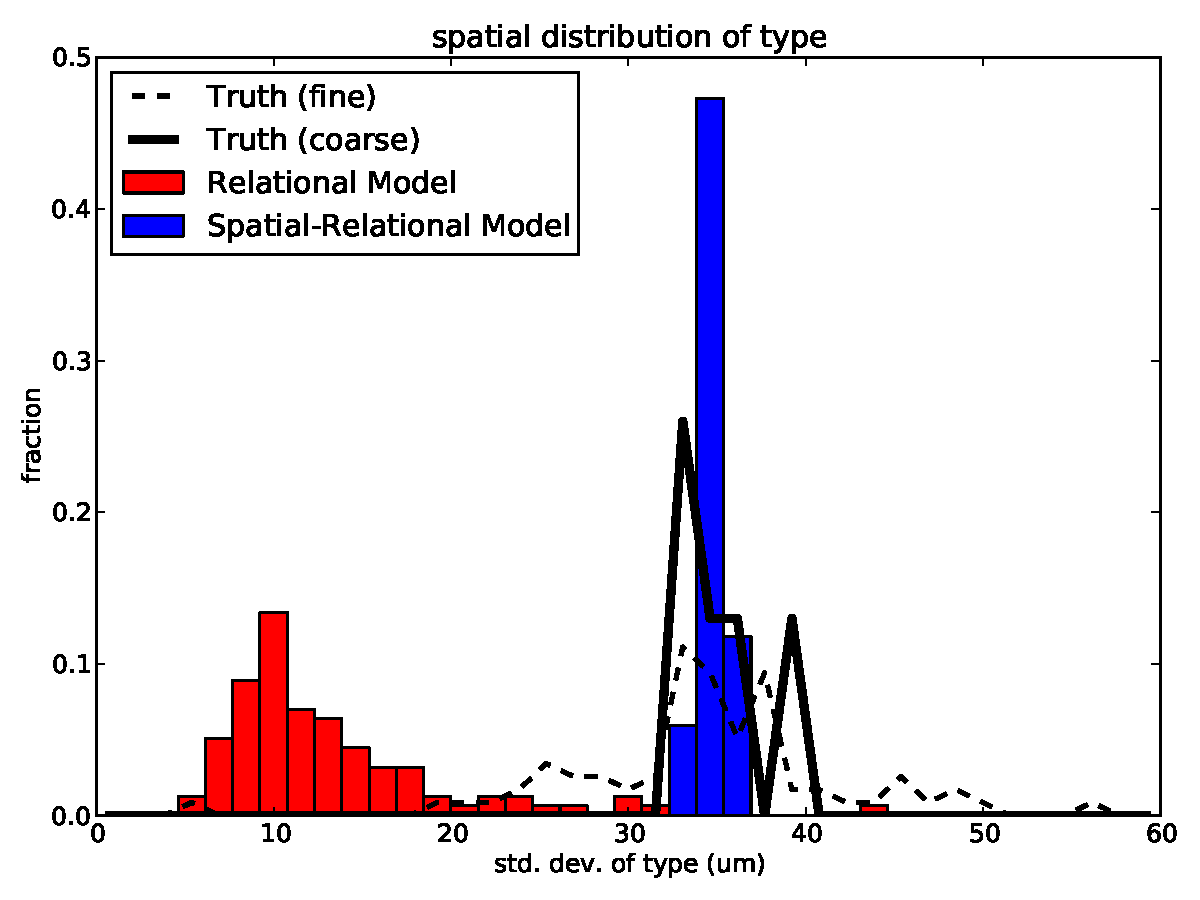
\includegraphics[width=5in]{mouseretina/spatial_var.pdf}}
  \caption{The distribution of the spatial extent of cell types found by each of
the above methods, and ground truth clusters}
\label{fig:supp:irmspatialcomparemouse}
\end{figure}

\begin{figure}[h!]
  \centering 
    \centerline{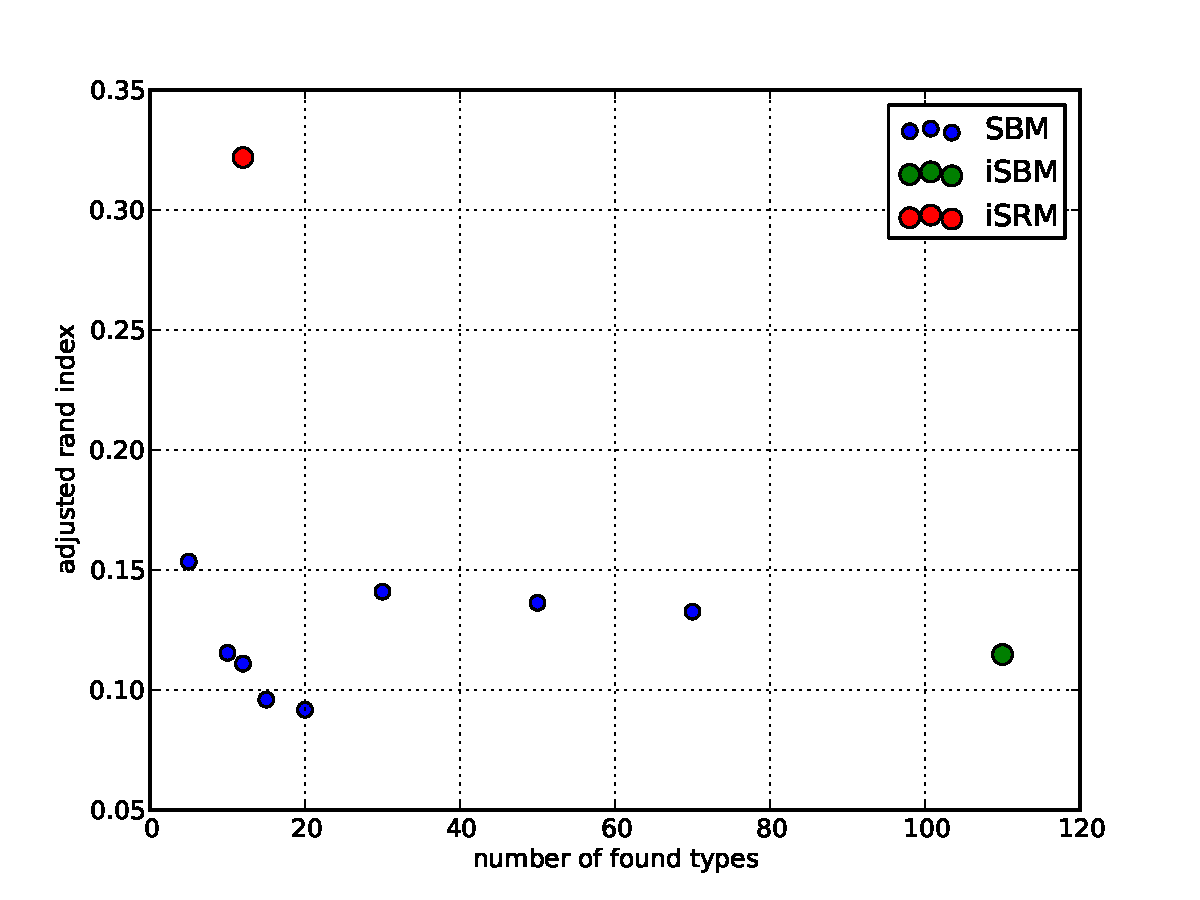
\includegraphics[width=5in]{mouseretina/ari_vs_cluster.pdf}}
  \caption{ARI vs cluster number for the iSRM, iSBM, and the SBM with varying K.}
\label{fig:supp:mousecompareari}
\end{figure}

\begin{figure}[h!]
  \centering 
    \centerline{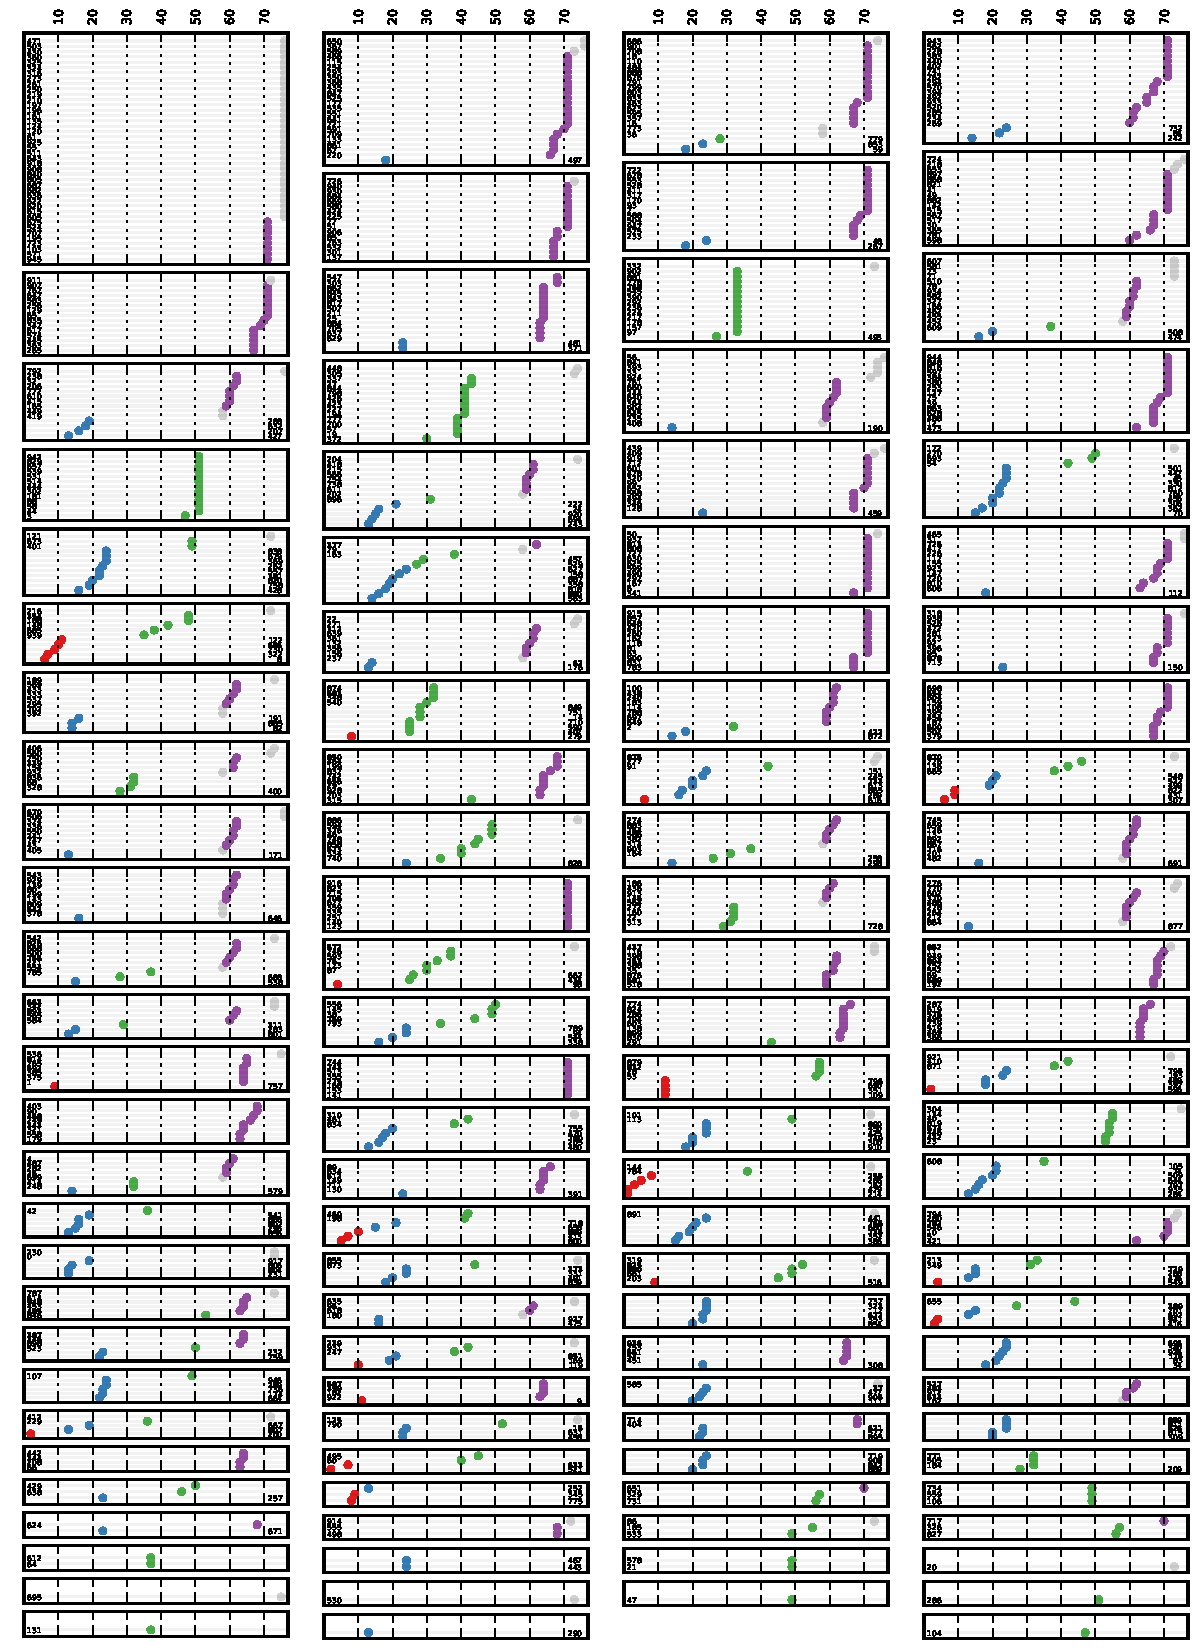
\includegraphics[width=6.0in]{mouseretina/retina.1.2.bb.0.0.data-fixed_20_100-anneal_slow_400.truth_latent.pdf}}
  \caption{The cell IDs and found types (grouped) vs known types (y-axis)  found by the infinite stochastic block model, dramatically overclustering relative to ground truth}
\label{fig:supp:retinabbclusters}
\end{figure}

\begin{figure}[h!]

  \centering 
    \centerline{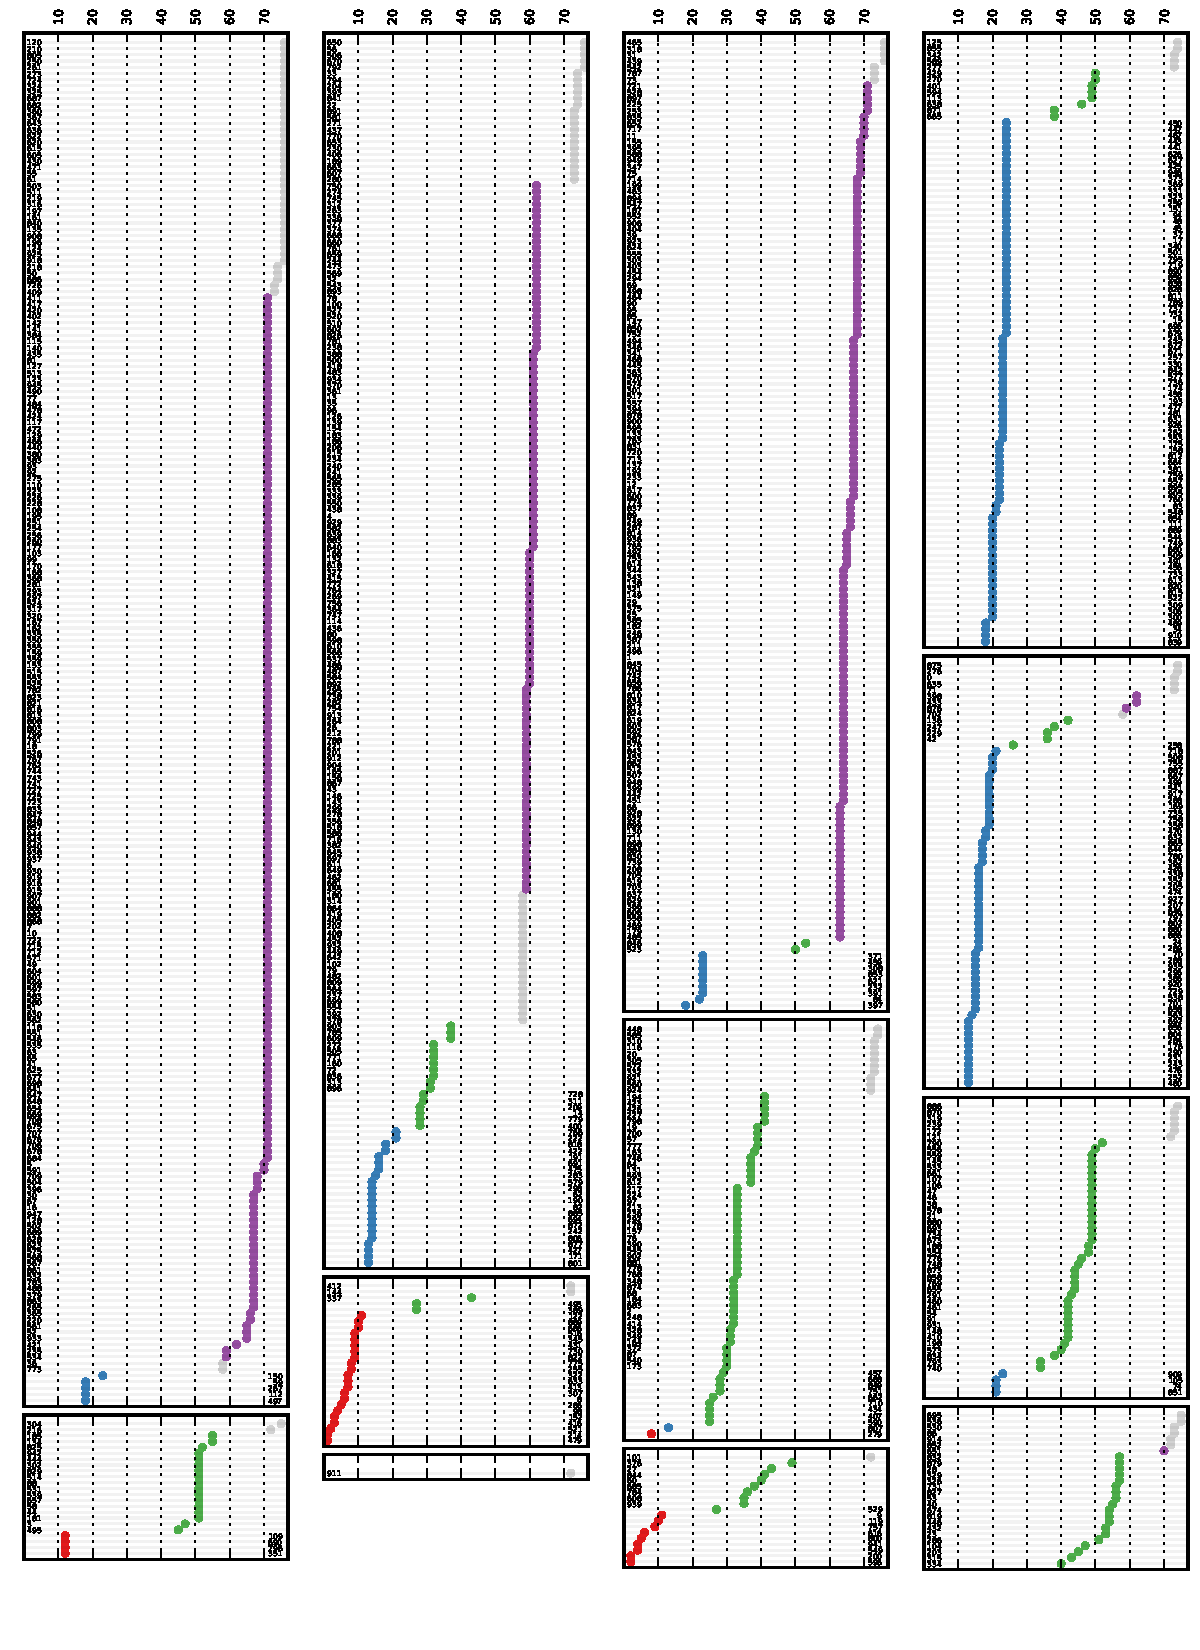
\includegraphics[width=6.0in]{mouseretina/retina.1.2.ld.0.0.data-fixed_20_100-anneal_slow_400.truth_latent.pdf}}
  \caption{The cell IDs and found types (grouped) vs known types (y-axis) by the infinite spatial-relational model.}
\label{fig:supp:retinaldclusters}
\end{figure}


\begin{figure}[h!]

  \centering 
    \centerline{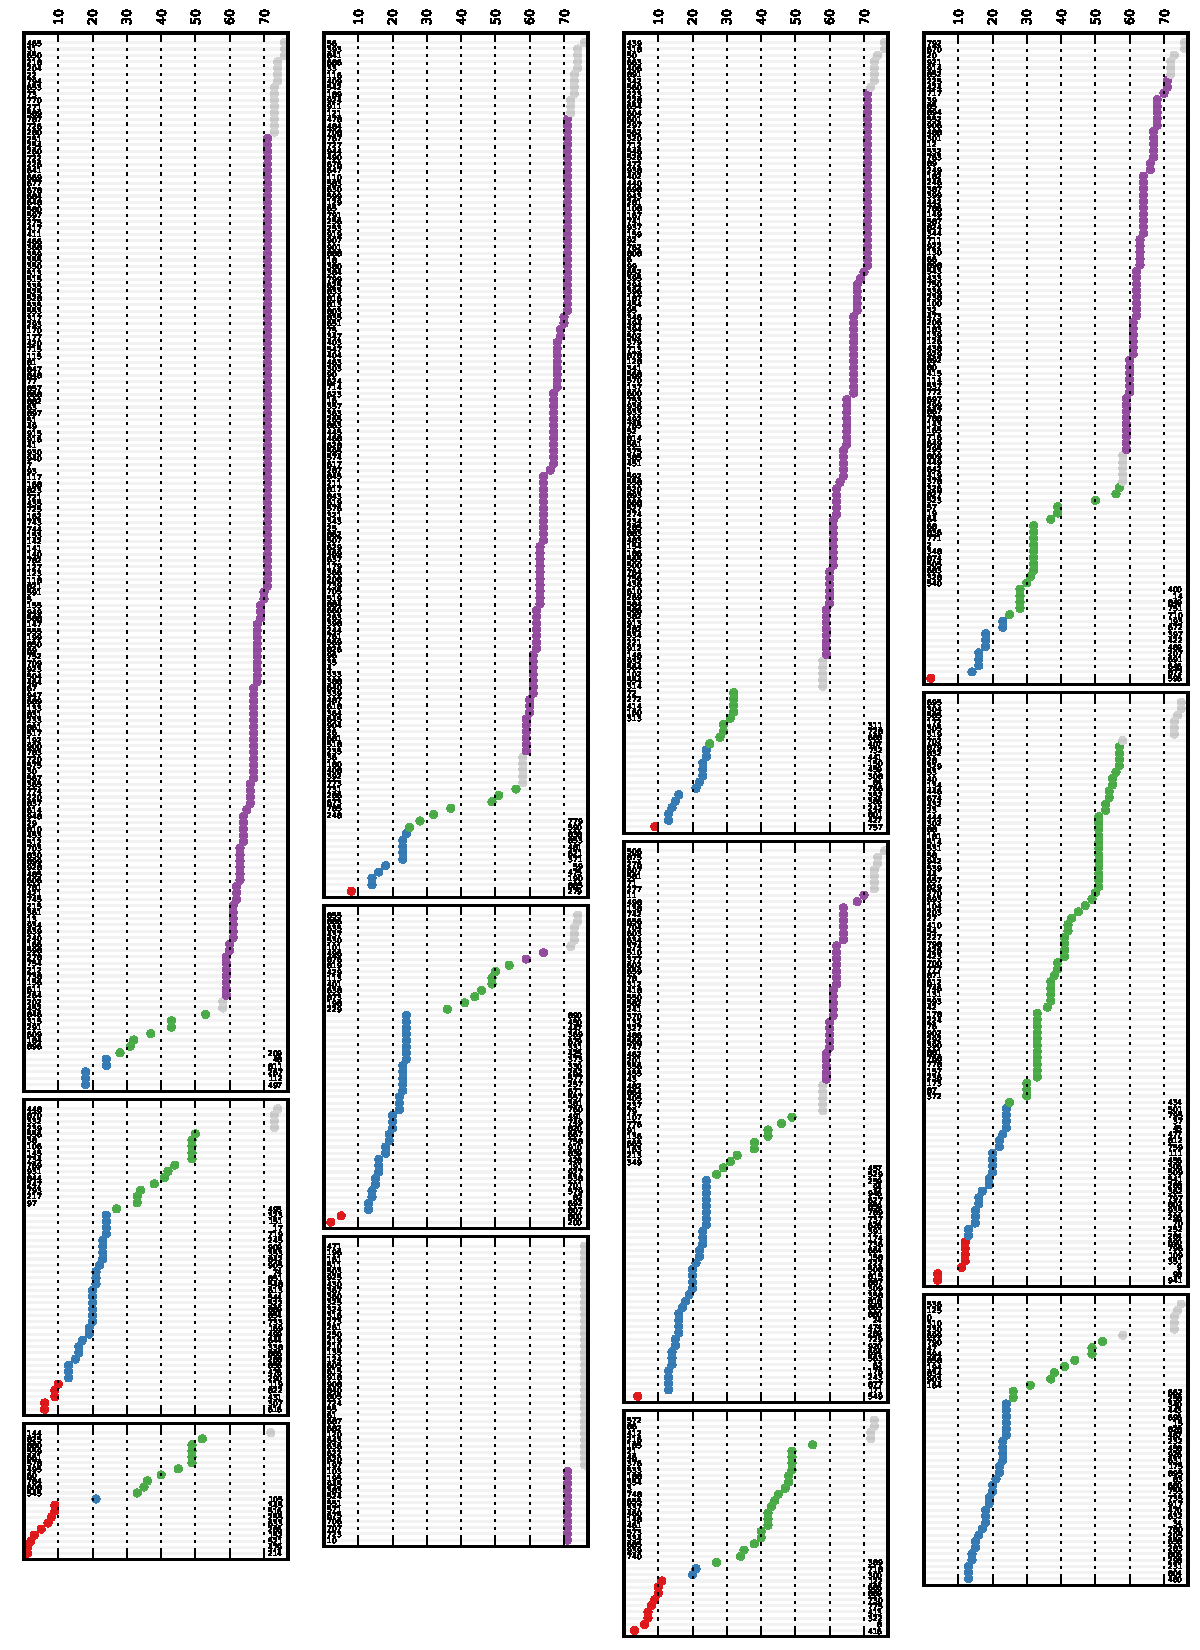
\includegraphics[width=6.0in]{mouseretina/retina.1.2.bb.0.0.data-fixed_20_12-anneal_slow_fixed_400.truth_latent.pdf}}
  \caption{The cell IDs and found types (grouped) vs known types (y-axis) via the stochastic block model with $k=12$}
\label{fig:supp:retinabbfixedclusters}
\end{figure}


\newpage

\FloatBarrier
\subsection{Hyperprior grids}
\label{supp:hyperpriors}

For the mouse retina Logistic-Distance Bernoulli model, we gridded $\mu^{hp}$ and $\lambda^{hp}$ into 40 $\log_{10}$-spaced points 1.0 and 80. $p_{min} \in [0.001, 0.005, 0.01]$ and $p_{max} \in [0.80, 0.90, 0.95, 0.99]$.

For the c. elegans data with the Logistic Distance poisson model, we gridded $\mu_{hp}$ and $\lambda$ into 20 $\log_{10}$-spaced points bween 0.2 and 2.0, and the $ratescale^{hp}$ parameter into 20 $\log_{10}$-spaced points between 2.0 and 20.0. We globally set $rate_{min}=0.01$. 

For the microprocessor with the Logistic Distance fixed lambda Bernoulli likelihood, we gridded $mu_{hp}$ into 50 $\log_{10}$-spaced points between 10 and 500 and set $\lambda=\mu_{hp}/10$. $p_{min} \in \{0.001, 0.01, 0.02\}$  and both $p_\alpha$ and $p_\beta \in \{0.1, 1.0, 2.0\}$. 


\section{Measuring clustering similarity}

The adjusted rand index (ARI) is a measure of the similarity of two
different clusterings \autocite{Hubert1985} -- two identical clusters
have an ARI of 1.0 while progressively more dissimilar clusters have
lower ARIs, becoming negative as the clustering gets anti-correlated.


\end{document}



